%--------------------------------------------------------------------
%Requisitos



\chapter{Requisitos}

Este capítulo apresenta o mapeamento dos requisitos do projeto.

\section{Problemas mapeados}

Para o estabelecimento de requisitos completos e coesos com os objetivos da solução foi executado o estudo de viabilidade (Apêndice \ref{appendix:estudo_viabilidade} que fomentou a criação do diagrama de causa e efeito (Figura \ref{fig:causa_e_efeito}). Os problemas foram categorizados em problemas de acesso, localização, carga e tempo.

\begin{figure}[hb]
		\centering
		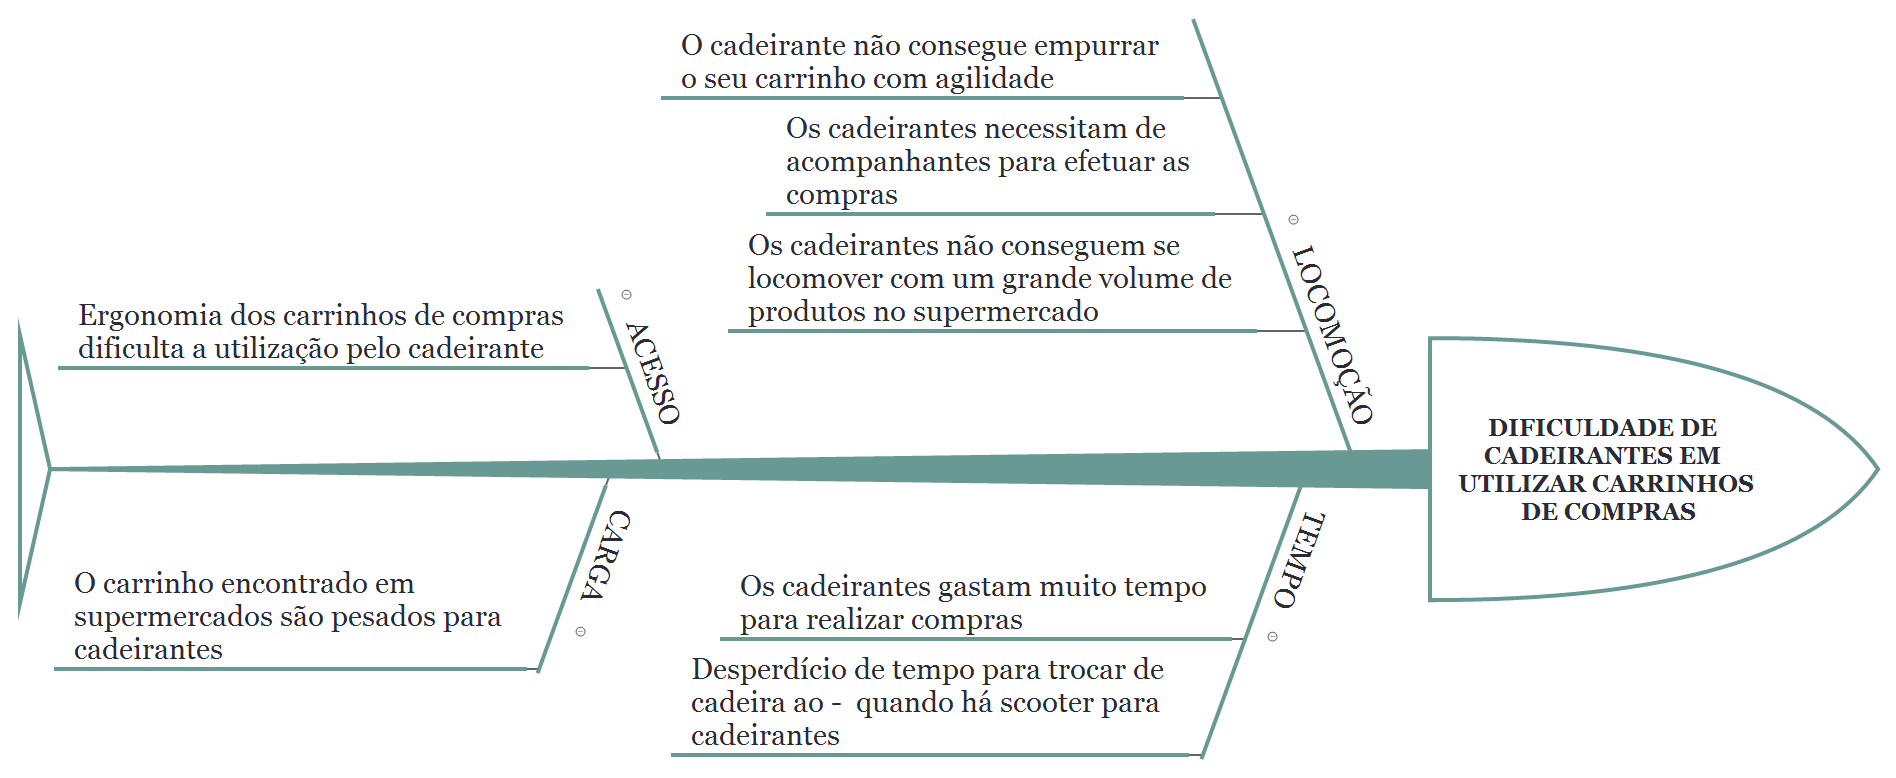
\includegraphics[width=1\textwidth]{figuras/diagramaefeito.png}
		\caption{Diagrama de Causa e Efeito. Fonte: Autores}
		\label{fig:causa_e_efeito}
\end{figure} 

\section{Requisitos funcionais}

A Tabela \ref{tab:req_func} apresenta os requisitos funcionais do produto e demonstra a dependência entre os mesmos além de promover a rastreabilidade dos problemas para a solução.  As categorias Locomoção, Acesso e Carga definidas pelo diagrama de causa e efeito são diretamente atacadas pelo requisito da solução. A categoria Tempo é indiretamente solucionada em todo o conjunto de requisitos.


% ######## init table ########
\begin{table}[h]
 \centering
 \caption{Requisitos funcionais do projeto} \label{tab:req_func}
% distancia entre a linha e o texto
 {\renewcommand\arraystretch{1.25}
 \begin{tabular}{ l l l l }
  \cline{1-1}\cline{2-2}\cline{3-3}\cline{4-4}  
    \multicolumn{1}{p{3.167cm}|}{\textbf{Categoria de Problemas}} &
    \multicolumn{1}{p{1.283cm}|}{\textbf{Id}} &
    \multicolumn{1}{p{4.783cm}|}{\textbf{Requisito}} &
    \multicolumn{1}{p{2.383cm}}{\textbf{Dependência}}
  \\  
  \cline{1-1}\cline{2-2}\cline{3-3}\cline{4-4}  
    \multicolumn{1}{p{3.167cm}|}{Locomoção} &
    \multicolumn{1}{p{1.283cm}|}{1} &
    \multicolumn{1}{p{4.783cm}|}{O carrinho deverá seguir o cadeirante de forma autônoma pelo supermercado considerando-se um ambiente ideal, ou seja, chão plano;} &
    \multicolumn{1}{p{2.383cm}}{2, 3, 4}
  \\  
  \cline{1-1}\cline{2-2}\cline{3-3}\cline{4-4}  
    \multicolumn{1}{p{3.167cm}|}{ } &
    \multicolumn{1}{p{1.283cm}|}{2} &
    \multicolumn{1}{p{4.783cm}|}{A distância entre o carrinho e o cadeirante será de 20 a 50cm;} &
    \multicolumn{1}{p{2.383cm}}{3}
  \\  
  \cline{1-1}\cline{2-2}\cline{3-3}\cline{4-4}  
    \multicolumn{1}{p{3.167cm}|}{ } &
    \multicolumn{1}{p{1.283cm}|}{3} &
    \multicolumn{1}{p{4.783cm}|}{O carrinho deverá ser capaz de desviar de obstáculos ao fazer curvas;} &
    \multicolumn{1}{p{2.383cm}}{ }
  \\  
  \cline{1-1}\cline{2-2}\cline{3-3}\cline{4-4}  
    \multicolumn{1}{p{3.167cm}|}{ } &
    \multicolumn{1}{p{1.283cm}|}{4} &
    \multicolumn{1}{p{4.783cm}|}{O cadeirante terá disponível um botão on/off para o carrinho;} &
    \multicolumn{1}{p{2.383cm}}{ }
  \\  
  \cline{1-1}\cline{2-2}\cline{3-3}\cline{4-4}  
    \multicolumn{1}{p{3.167cm}|}{Acesso} &
    \multicolumn{1}{p{1.283cm}|}{5} &
    \multicolumn{1}{p{4.783cm}|}{O carrinho deverá conter o espaço/estrutura necessária para o cadeirante colocar suas compras;} &
    \multicolumn{1}{p{2.383cm}}{ }
  \\  
  \cline{1-1}\cline{2-2}\cline{3-3}\cline{4-4}  
    \multicolumn{1}{p{3.167cm}|}{ } &
    \multicolumn{1}{p{1.283cm}|}{6} &
    \multicolumn{1}{p{4.783cm}|}{A estrutura do carrinho deve atender as medidas necessárias para o alcance do cadeirante} &
    \multicolumn{1}{p{2.383cm}}{ }
  \\  
  \cline{1-1}\cline{2-2}\cline{3-3}\cline{4-4}  
    \multicolumn{1}{p{3.167cm}|}{ } &
    \multicolumn{1}{p{1.283cm}|}{7} &
    \multicolumn{1}{p{4.783cm}|}{A posição do carrinho parado e/ou em movimento deve ser acessível ao cadeirante} &
    \multicolumn{1}{p{2.383cm}}{3, 7}
  \\  
  \cline{1-1}\cline{2-2}\cline{3-3}\cline{4-4}  
    \multicolumn{1}{p{3.167cm}|}{Carga} &
    \multicolumn{1}{p{1.283cm}|}{8} &
    \multicolumn{1}{p{4.783cm}|}{O carrinho terá um peso total de até 50kg, reservando-se 20kg para compras.} &
    \multicolumn{1}{p{2.383cm}}{ }
  \\  
  \hline

 \end{tabular} }
\end{table}


\subsection{Requisitos não funcionais}

Os requisitos não funcionais definidos para a solução são listados abaixo:

\begin{itemize}
\item O carrinho terá velocidade máxima de 5km/h;
\item O carrinho terá autonomia de até 2 horas;
\item O carrinho deverá ser utilizado somente dentro do mercado, pelo cadeirante;
\item O carrinho poderá ser recarregável;
\item O carrinho será de propriedade do mercado, que o usará como adicional para necessidades especiais;
\item O cadeirante deverá ser instruído a andar devagar para que o carrinho consiga acompanhá-lo.
\end{itemize}




